\chapter{算法分析及系统架构设计}
本章将针对循环神经网络前向传播过程提出一套从软件算法,硬件实现到系统集成的全流程设计框架和独立整的解决方案。不同于所有过往的压缩加速设计,
本文所采用的压缩算法具有压缩成本小,无需训练集等优势,可以不依赖云端算力支持,仅在分布式的边缘设备实现,算法的详细介绍将在3.1节展开。算法特性
决定了其适用场景,而具有弹性性能需求的应用场景又是普遍存在的,所以在现实条件的约束下,本文对算法进行了合理的拆分与协同并分别映射到软件和硬件上
进行执行,具体的系统架构设计见3.2节。最后,面向算法和应用场景需求,本文进行了定制化专用硬件架构的设计,通过对上层应用的需求和硬件加速空间
进行分析,本文创造性的提出了一种具有紧凑计算结构和可配置功能模块的循环神经网络前向传播硬件加速器。该加速器能通过简单的配置和数据重载完成不同网络结构
和不同模型大小的切换,相比传统的神经网络加速器的一种硬件实现对应唯一的网络结构和模型尺寸,本文所设计的加速器即具有“专用”所带来的高效性,
又具有一定程度“通用”所带来的灵活性,能满足弹性应用场景下性能可调的需求。在众多的循环神经网络模型中,本文选取回声状态网络作为设计实例,因其结构简单,
训练成本低和应用前景开阔等优势,同时又极具代表性和紧迫性,详细分析说明可见2.1节。对于其他种类的循环神经网络,除具体实现细节存在微小差异外,本文在
系统层面提出的设计方案,软件算法和硬件架构设计也同样适用,因此,本文不再一一说明。
\section{基于投影的模型压缩算法}
本小节先展示模型压缩的效果---简化网络结构,然后就简化网络的生成过程(状态投影和激活函数近似)作详细的说明,最后会评估与分析压缩算法的特性和作用效果。
以上描述的模型压缩的全景图是本文后续工作的基础。
\subsection{简化网络结构}
回声状态网络在模型压缩算法的作用下生成了简化网络,其数学模型为式\ref{eq:redesn},式中\(\widehat{x},\widehat{z} \in \mathbb{R}^q\)表示简化网络隐藏层的状态,
\(\widehat{W}, \widehat{E}_d \in \mathbb{R}^{q \times q}\)表示隐藏层与隐藏层的连接权重,\(\widehat{E}_l,\in \mathbb{R}^{q \times q}\)表示隐藏层跨时间步的自循环矩阵,
\(\widehat{W}_{in},\widehat{W}_{out}\in \mathbb{R}^{q \times n_{in}}\)分别表示输入到隐藏层以及隐藏层到输出的连接权重,\(q\)是隐藏层的神经元数量,
\(n_{in}\)为输入数量,\(n_{out}\)为输出数量。
\begin{equation}\label{eq:redesn}
	\begin{split}
		\widehat{z}_t &= f(\widehat{W} * \widehat{x}_{t-1} + \widehat{W}_{in} * u_{t})				\\	
		\widehat{x}_t &= \widehat{E}_l * \widehat{x}_{t-1} + \widehat{E}_d * \widehat{z}_{t} 		\\
		y_{t} 			&= \widehat{W}_{out} * \widehat{x}_{t}	
	\end{split}
\end{equation}

相较于回声状态网络的原网络模型,简化网络的数学描述更加复杂, 具体表现为引入了新的状态变量\(\widehat{z}\)和新的新的拓扑连接\(\widehat{E}_l,\widehat{E}_d\)。
\(\widehat{z}\)是输入\(u\)和状态\(\widehat{x}\)的函数,而\(\widehat{x}\)又与暂态\(\widehat{z}\)呈线性相关的关系。这些新引入的变量和关系
改变了回声状态网络的模型结构,即简化网络在原网络结构的基础上增加了一层隐藏层,如图\ref{fig:esn_convert}所示。此外,简化网络拥有两个循环结构:暂态\(\widehat{z}\)
和状态\(\widehat{x}\)之间的层间循环体和状态层\(\widehat{x}\)内部的自循环体。循环体的增加赋予了循环神经网络更强大的记忆能力,这使得少量的隐藏层神经元
就可以实现对系统动态特性的表征。显然,本文所采用的模型压缩算法在网络结构上做出了让步,但是“祸兮,福之所倚”,简化网络在压缩神经元数量方面取得了巨大的成功。
二者利害相权的最终结果是:在模型预测精度不显著下降的情况下,简化网络的参数量将大幅减少,前向传播过程的时间复杂度也显著降低。
\begin{figure}
	\centering
	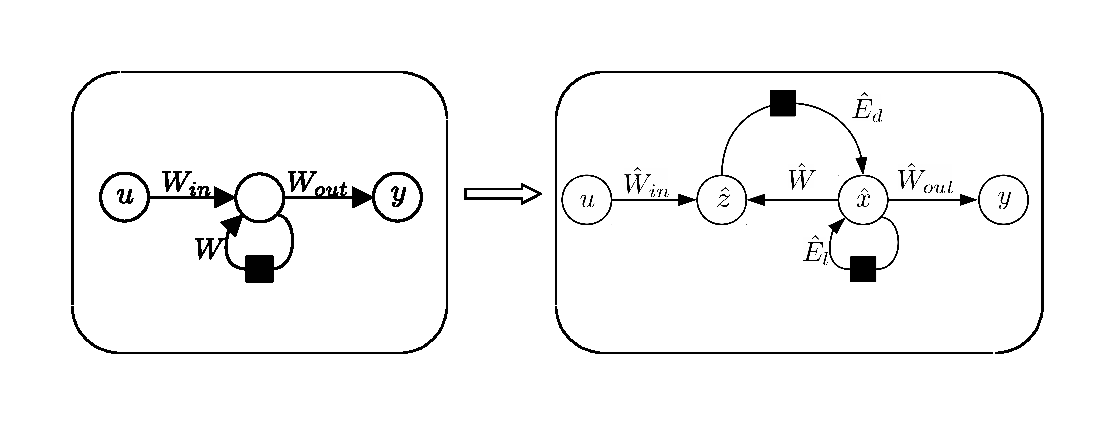
\includegraphics[width=0.7\columnwidth]{ESN_convert.eps}
	\caption{原始网络和简化网络的结构图}
	\label{fig:esn_convert}
\end{figure}

回声状态网络的回路结构如图\ref{fig:esn_red}所示。
复杂度分析

结构相似性分析

\begin{figure}
	\centering
	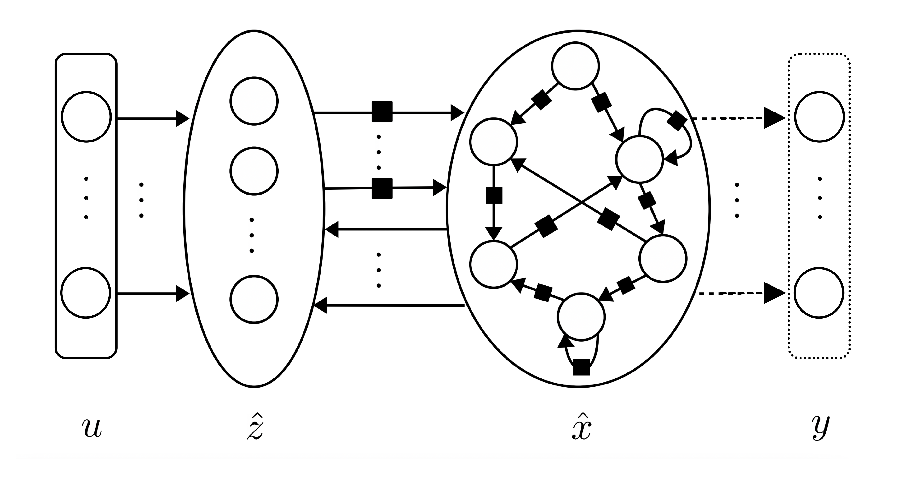
\includegraphics[width=0.7\columnwidth]{ESN_red.eps}
	\caption{简化回声状态网络结构}
	\label{fig:esn_red}
\end{figure}

\subsection{本征正交分解与离散经验插值}
介绍高速回声状态网络的生成,算法顺序介绍,or硬件需求倒推
\subsection{压缩算法的评估与分析}
从精度和复杂度方面分析。

\section{系统整体架构设计}
应用场景介绍引入软硬件功能划分。
\subsection{前向传播及压缩流程}
\subsection{软硬件功能划分}
\subsection{系统整体架构}

\section{面向算法的定制化硬件分析}
\subsection{算法需求分析}
1需要实现原始网络,高速网络两个网络结构。
2压缩网络结构尺寸可调节。
3模型压缩过程。
\subsection{硬件模块划分与复用性分析}
\subsection{激活函数分段近似}
\subsection{计算资源与存储资源需求分析}

\section{基于FPGA的加速器设计}
\subsection{硬件加速器整体架构}

\subsection{存储架构设计}

\subsection{计算架构设计}

\subsection{矩阵向量乘法模块}

\subsection{激活函数模块}

\subsection{IP核互联设计}

\section{本章小结}
